\documentclass{khlexamen}
\usepackage[dutch]{babel}
\usepackage{tikz}
\usepackage{xfrac}

\newcommand{\academiejaar}{2013--2014}
\newcommand{\examendatum}{22 augustus 2014}
\newcommand{\beginuur}{8.30}
\newcommand{\opleiding}{Bachelor in de Toegepaste Informatica}
\newcommand{\fase}{1}
\newcommand{\activiteit}{Examen Augustus}
\newcommand{\opo}{MBI04A -- Algoritmen en datastructuren 1}
\newcommand{\ola}{MBI04A -- Algoritmen en datastructuren 1}

\newcommand{\hulpmiddelen}{Geen}
\newcommand{\examinator}{F. Vogels}
\newcommand{\duur}{3 uur}


\usetikzlibrary{calc}

\makeatletter\newcommand{\minuscule}{\@setfontsize\miniscule{4}{5}}\makeatother

\newcommand{\emptygrid}[2]{
  \pgfmathparse{#1/2}\let\maxx\pgfmathresult
  \pgfmathparse{#2/2}\let\maxy\pgfmathresult
  \foreach \x in {0,0.5,...,\maxx} {
    \draw[thin] (\x,0) -- (\x,\maxy);
  }
  \foreach \y in {0,0.5,...,\maxy} {
    \draw[thin] (0,\y) -- (\maxx,\y);
  }
}

\newcommand{\emptybiggrid}[2]{
  \pgfmathparse{#1}\let\maxx\pgfmathresult
  \pgfmathparse{#2}\let\maxy\pgfmathresult
  \foreach \x in {0,...,\maxx} {
    \draw[thin] (\x,0) -- (\x,\maxy);
  }
  \foreach \y in {0,...,\maxy} {
    \draw[thin] (0,\y) -- (\maxx,\y);
  }
}

\begin{document}

\HEADER

\guidelines

\oralpart

\clearpage


\section{Schriftelijk Deel}
\begin{center}
\framebox{\Large {\bf Drie uur} na aanvang van het examen wordt je kopij opgehaald.}
\end{center}

\subsection{Recursie}
Schrijf een \emph{recursieve} functie {\tt zeros} die telt op hoeveel nullen een gegeven getal eindigt.
\paragraph{Voorbeeld}
\begin{center}
  \begin{tabular}{ll}
    {\tt n} & {\tt zeros(n)} \\
    \toprule
    0 & 1 \\
    10 & 1 \\
    200 & 2 \\
    5000 & 3 \\
    1001 & 0 \\
    10010 & 1
  \end{tabular}
\end{center}

\vskip4mm
\answerlines[14]

\clearpage
\SMALLHEADER
\subsection{2048}
Voor deze opgave implementeren we de basisfunctionaliteit voor het spel 2048. Kennis van dit spel is
uiteraard niet vereist.

\subsubsection{{\tt createGrid}}
Schrijf een functie {\tt createGrid(width, height, init)} die een grid (rooster)
aanmaakt met breedte {\tt width} en hoogte {\tt height}. Elk element moet ge\"initialiseerd worden
op de waarde {\tt init}. Stel de grid voor als een array van kolommen, m.a.w. zodat je {\tt grid[x][y]}
kan gebruiken om het element in kolom {\tt x} en rij {\tt y} op te vragen.

\paragraph{Voorbeeld}
{\tt createGrid(4, 2, 0)} genereert {\tt [[0,0],[0,0],[0,0],[0,0]]}
hetgeen deze grid voorstelt:
\[
\begin{array}{|c|c|c|c|}
  \hline
    0 & 0 & 0 & 0 \\
  \hline
    0 & 0 & 0 & 0 \\
  \hline
\end{array}
\]

\vskip4mm
\answerlines[12]

\clearpage
\subsubsection{{\tt width} \& {\tt height}}
Schrijf functies {\tt width} en {\tt height} die resp.\ de breedte en hoogte van een grid teruggeven.

\paragraph{Voorbeeld}
\begin{center}
\begin{minipage}{.8\linewidth}
\begin{lstlisting}[language=javascript]
var grid = createGrid(5, 3, 1);
width(grid) // 5
height(grid) // 3
\end{lstlisting}
\end{minipage}
\end{center}

\vskip4mm
\answerlines[17]

\clearpage
\SMALLHEADER
\subsubsection{{\tt slideOne}}
In het spel 2048 hebben we te maken met een grid waarvan de vakjes
ofwel leeg zijn (stellen we voor d.m.v.\ {\tt null}), ofwel een getal bevatten.

\begin{center}
  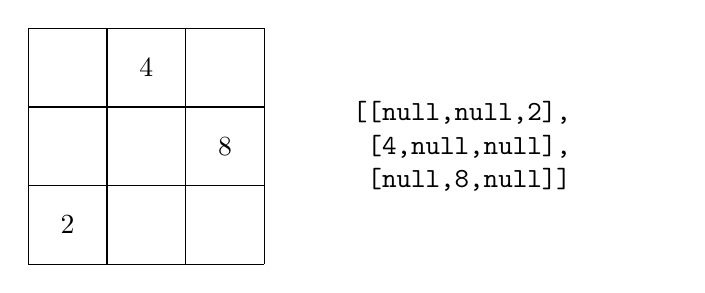
\begin{tikzpicture}
    \draw (0,0) grid (3,3);
    \node at (.5,.5) {2};
    \node at (1.5,2.5) {4};
    \node at (2.5,1.5) {8};

    \node[anchor=west] at (4,1.5) {\parbox{4cm}{\tt
      [[null,null,2], \\{}\phantom{x}[4,null,null], \\{}\phantom{x}[null,8,null]]
    }
    };
  \end{tikzpicture}
\end{center}

De oproep {\tt slideOne(grid, x, y)} schuift het getal op positie ({\tt x}, {\tt y}) naar
links volgens de volgende regels:
\begin{itemize}
  \item Het getal verschuift naar links zolang de vakjes leeg zijn.
  \item Indien het getal tegen de linkerrand botst, blijft het daar gewoon staan.
    \begin{center}
      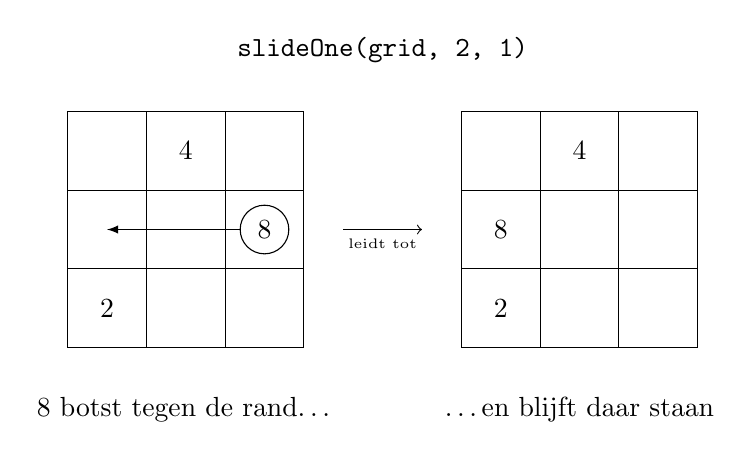
\begin{tikzpicture}
        \node[anchor=south] at (4,3.5) {\tt slideOne(grid, 2, 1)};

        \begin{scope}
          \draw (0,0) grid (3,3);
          \node at (.5,.5) {2};
          \node at (1.5,2.5) {4};
          \node[circle,draw] (shifted) at (2.5,1.5) {8};
          \draw[-latex] (shifted) -- (0.5,1.5);
          \node[anchor=north] at (1.5,-.5) {8 botst tegen de rand\dots};
        \end{scope}

        \draw[->] (3.5,1.5) -- +(1,0) node[midway,below,font=\tiny] {leidt tot};

        \begin{scope}[xshift=5cm]
          \draw (0,0) grid (3,3);
          \node at (.5,.5) {2};
          \node at (1.5,2.5) {4};
          \node at (0.5,1.5) {8};
          \node[anchor=north] at (1.5,-.5) {\dots en blijft daar staan};
        \end{scope}

      \end{tikzpicture}
    \end{center}
  \item Indien het botst tegen een \emph{ongelijk} getal, blijft het daar staan.
    \begin{center}
      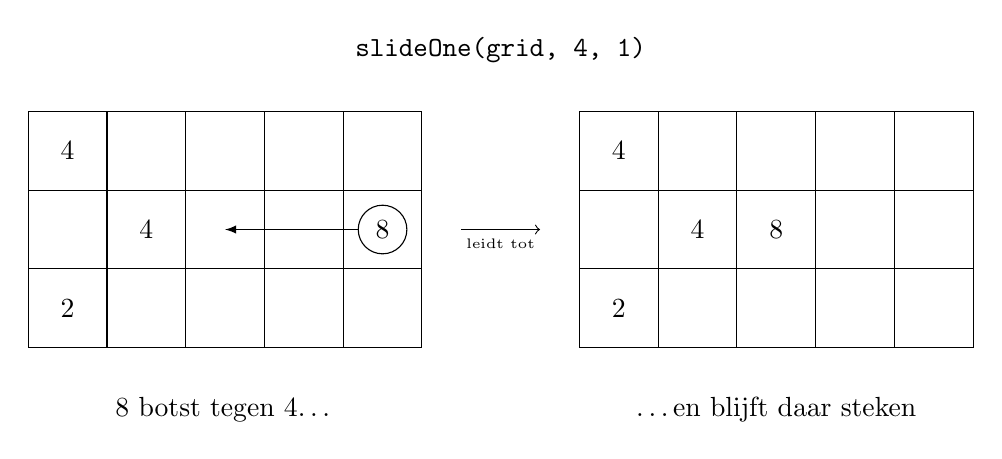
\begin{tikzpicture}
        \node[anchor=south] at (6,3.5) {\tt slideOne(grid, 4, 1)};

        \begin{scope}
          \draw (0,0) grid (5,3);
          \node at (.5,.5) {2};
          \node at (0.5,2.5) {4};
          \node at (1.5,1.5) {4};
          \node[circle,draw] (shifted) at (4.5,1.5) {8};
          \draw[-latex] (shifted) -- (2.5,1.5);
          \node[anchor=north] at (2.5,-.5) {8 botst tegen 4\dots};
        \end{scope}

        \draw[->] (5.5,1.5) -- +(1,0) node[midway,below,font=\tiny] {leidt tot};

        \begin{scope}[xshift=7cm]
          \draw (0,0) grid (5,3);
          \node at (.5,.5) {2};
          \node at (0.5,2.5) {4};
          \node at (1.5,1.5) {4};
          \node at (2.5,1.5) {8};
          \node[anchor=north] at (2.5,-.5) {\dots en blijft daar steken};
        \end{scope}
      \end{tikzpicture}
    \end{center}
    \clearpage
  \item Indien het botst tegen een \emph{gelijk} getal, fusioneren ze met elkaar
        en bevat de grid op die plaats de som van de getallen.
    \begin{center}
      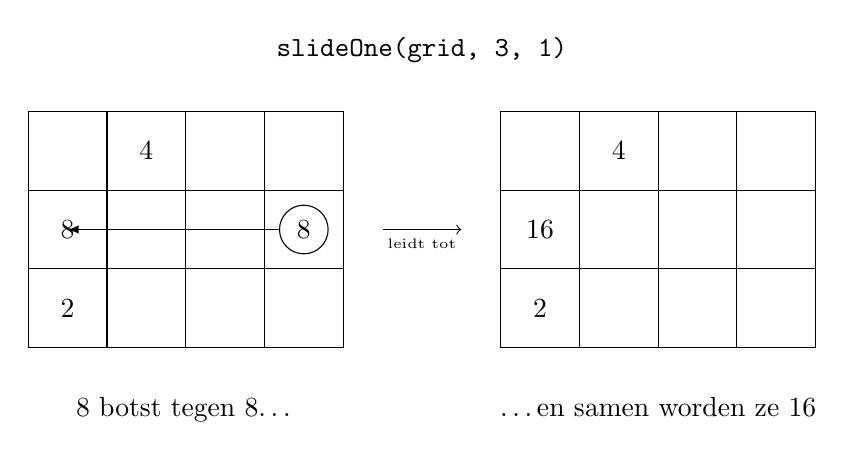
\begin{tikzpicture}
        \node[anchor=south] at (5,3.5) {\tt slideOne(grid, 3, 1)};

        \begin{scope}
          \draw (0,0) grid (4,3);
          \node at (.5,.5) {2};
          \node at (1.5,2.5) {4};
          \node at (0.5,1.5) {8};
          \node[circle,draw] (shifted) at (3.5,1.5) {8};
          \draw[-latex] (shifted) -- (0.5,1.5);
          \node[anchor=north] at (2,-.5) {8 botst tegen 8\dots};
        \end{scope}

        \draw[->] (4.5,1.5) -- +(1,0) node[midway,below,font=\tiny] {leidt tot};

        \begin{scope}[xshift=6cm]
          \draw (0,0) grid (4,3);
          \node at (.5,.5) {2};
          \node at (1.5,2.5) {4};
          \node at (0.5,1.5) {16};
          \node[anchor=north] at (2,-.5) {\dots en samen worden ze 16};
        \end{scope}
      \end{tikzpicture}
    \end{center}
\end{itemize}

\vskip4mm
\answerlines[15]

\clearpage
\ANSWERPAGE

\clearpage
\subsubsection{{\tt slideAll}}
Schrijf de functie {\tt slideAll(grid)} die {\tt slideOne(grid, x, y)} toepast
op elk getal in de grid, te beginnen met de rechterkolom en zo naar links.
Als getallen in dezelfde kolom zitten, maakt de volgorde niet uit.

\paragraph{Voorbeeld}
\begin{center}
  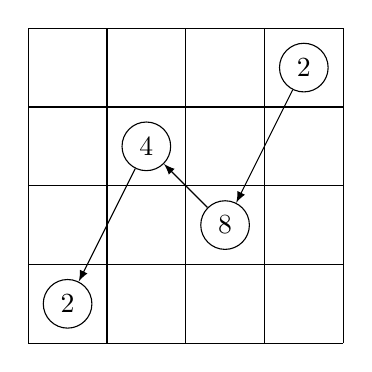
\begin{tikzpicture}
    \draw (0,0) grid (4,4);
    \node[draw,circle] (c1) at (.5,.5) {2};
    \node[draw,circle] (c2) at (1.5,2.5) {4};
    \node[draw,circle] (c3) at (2.5,1.5) {8};
    \node[draw,circle] (c4) at (3.5,3.5) {2};

    \draw[-latex] (c4) -- (c3);
    \draw[-latex] (c3) -- (c2);
    \draw[-latex] (c2) -- (c1);
  \end{tikzpicture}
\end{center}
In dit voorbeeld wordt eerst de rechter {\tt 2} verschoven, vervolgens
de {\tt 8}, dan de {\tt 4} en uiteindelijk de linker {\tt 2}.

\vskip8mm
\answerlines[13]


\clearpage
\ANSWERPAGE

\subsubsection{{\tt rotateCounterClockwise}}
Gegeven is de functie {\tt rotateClockwise(grid)} die een grid een kwartslag in wijzerzin draait.
\begin{center}
\begin{minipage}{.8\linewidth}
\begin{lstlisting}[language=javascript]
function rotateClockwise(grid)
{
    var w = width(grid);
    var h = height(grid);

    var result = createGrid( h, w );

    for ( var x = 0; x !== w; ++x )
    {
        for ( var y = 0; y !== h; ++y )
        {
            result[h-y-1][x] = grid[x][y];
        }
    }

    return result;
}
\end{lstlisting}
\end{minipage}
\end{center}

\paragraph{Voorbeeld}
\[
  \begin{array}{ccc}
    1 & 2 & 3 \\
    4 & 5 & 6 \\
    7 & 8 & 9 \\
  \end{array}
  \quad\rightarrow\quad
  \begin{array}{ccc}
    7 & 4 & 1 \\
    8 & 5 & 2 \\
    9 & 6 & 3 \\
  \end{array}
\]

Schrijf nu de functie {\tt rotateCounterClockwise(grid)} die een grid
een kwartslag in \emph{tegenwijzerzin} draait.

\vskip4mm
\answerlines[8]
\clearpage
\ANSWERPAGE
\clearpage
\answerlines

\end{document}